% ===== CHAPTER 12 =====
\chapter{分子对称性}
\label{chap:12}
\section{对称元素和对称操作}
\label{sec:12.1 Symmetry Elements and Symmetry Operations}

    分子波函数和性质的定性信息通常可通过分子的对称性获得。所谓分子的对称性，指的是由处于平衡位置的核所形成的框架的对称性。（分子量子力学的起点是玻恩-奥本海默近似，该近似在求解电子波函数时将核视为固定；参见第\ref{sec:13.1 The Born-Oppenheimer Approximation}节。）分子的对称性在不同电子态下可能不同。例如，\ce{HCN}分子在基态下为线性，但在某些激发态下为非线性。除非另有说明，我们将考虑基态的对称性。

\subsection*{对称元素和对称操作}

    \textbf{对称操作}（symmetry operation）是对物体进行的变换，使得最终位置与初始位置在物理上无法区分，且物体中所有点对之间的距离保持不变。例如，考虑三角平面分子\ce{BF_3}（图\ref{fig:12.1}a），为了方便起见，我们对氟原子核进行了编号。如果我们以通过硼原子核且垂直于分子平面的轴为旋转轴，将分子逆时针旋转$120°$，则新位置如图\ref{fig:12.1}b所示。由于实际上氟原子核在物理上无法区分，我们已完成了一次对称变换。我们旋转分子的轴是一个对称元素的例子。对称元素和对称操作是相关但不同的概念，常常被混淆。\textbf{对称元素}（symmetry element）是进行对称操作的几何实体（点、线或面）。

    若将某物体绕某轴旋转$360/n$度（其中$n$是整数），得到与原始位置在物理上无法区分的构型，我们说该物体具有\textbf{$n$重对称轴}（$n$-fold axis of symmetry）（也称为\textit{$n$重主轴或$n$重旋转轴}）；其中$n$称为该轴的\textit{阶}（order）。例如，分子\ce{BF_3}在有一根三重对称轴垂直于分子所在平面。一般将$n$重旋转轴记作$C_n$。那么\ce{BF_3}中的三重对称轴可记作$C_3$轴。为了表示逆时针旋转$\left(360/n\right)°$的操作，我们使用$\hat{C}_n$来表示。“帽子”用于区分对称操作与对称元素。\ce{BF_3}有多于三根旋转轴，每根\ce{B-F}键的轴都是两重对称轴（图\ref{fig:12.2}）。
    \begin{figure}[ht!]
        \centering
        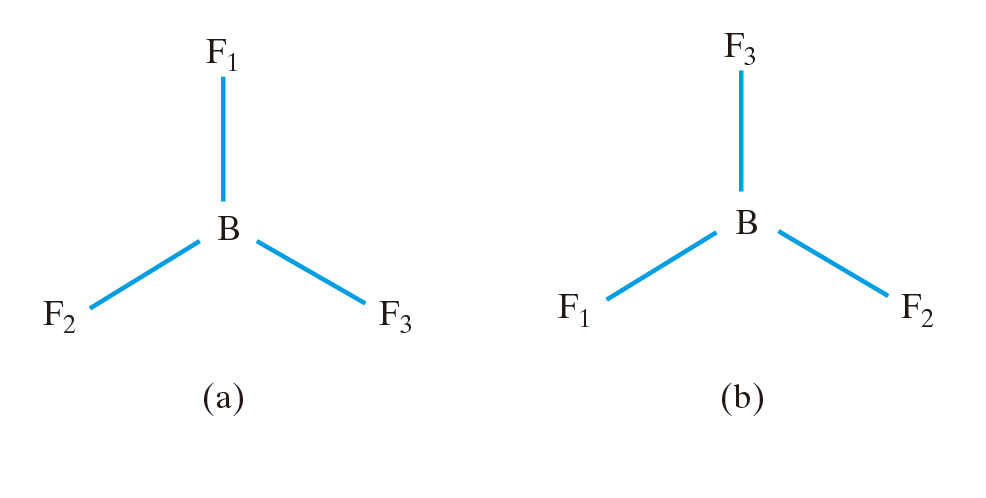
\includegraphics[width=0.5\textwidth]{Figures/12.1.png}
        \caption{
            \centering
            \parbox{0.4\textwidth}{
                \noindent
                (a)\ce{BF_3}分子。(b)通过硼原子垂直于分子所在平面的旋转轴旋转$120°$后的分子。
            }
        }
        \label{fig:12.1}
    \end{figure}
    \begin{figure}[ht!]
        \centering
        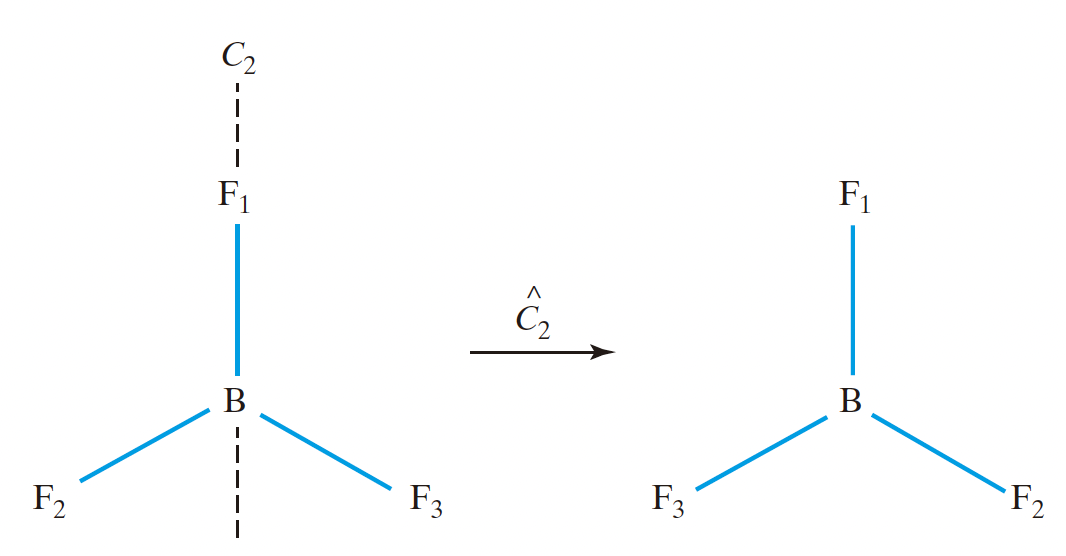
\includegraphics[width=0.5\textwidth]{Figures/12.2.png}
        \caption{\ce{BF_3}分子中的一根$C_2$轴。}
        \label{fig:12.2}
    \end{figure}

    第二种对称元素是\textbf{对称平面}（plane of symmetry）。如果所有原子核通过该平面反映后，其构型与原始构型在物理上无法区分，则该分子具有对称平面。对称平面的符号为 $\sigma$（小写希腊字母 sigma）。（\textit{Spiegel}是德语中“镜子”的意思。）反映对称操作记为$\hat{\sigma}$。\ce{BF_3}有四个反映面。分子所在平面是一个反映面，因为位于反映面的原子核在进行反映时不会移动。通过\ce{B}和\ce{F_1}核且与分子所在平面垂直的平面也是一个反映面，因为通过该平面反映仅交换了\ce{F_2}和\ce{F_3}。可能有人认为该反映操作与绕通过\ce{B}和\ce{F_1}的$C_2$轴旋转$180°$（也交换了\ce{F_2}和\ce{F_3}）相同。但事实并非如此。反映将位于分子平面上方的点映射到同样位于分子平面上方的点，而$C_2$旋转则将位于分子平面上方的点映射到位于分子平面下方的点。\textit{两个对称操作只有在它们表示三维空间的同一变换时才相等。}\ce{BF_3}中剩下的两个反映面为通过\ce{B-F_2}和\ce{B-F_3}核且与分子所在平面垂直的两个平面。

    第三种对称元素是\textbf{对称中心}（center of symmetry），用$i$表示（与$\sqrt{-1}$没有关系）。如果通过对称中心反演所有原子核的操作得出的构型与原始构型无法区分，则该分子具有对称中心。如果建立一个笛卡尔坐标系，则通过原点（用 $\hat{i}$ 表示）进行反演操作将原本位于 $\left(x, y, z\right)$ 的原子核转移到 $\left(−x, −y, −z\right)$。\ce{BF_3}有对称中心吗？以硼原子核为原点，反演过程得到如图\ref{fig:12.3}所示的结果。由于我们得到了与原始构型在物理上截然不同的构型，因此 \ce{BF_3} 没有对称中心。\ce{SF_6}通过硫原子核的反演过程如图\ref{fig:12.4}所示，可以清楚地看到\ce{SF_6}具有对称中心。（如$\hat{i}$或$\hat{C}_n$的操作可能是也可能不是对称操作。因此，$\hat{i}$是\ce{SF_6}中的一个对称操作而不是\ce{BF_3}中的。）
    \begin{figure}[htbp]
        \centering
        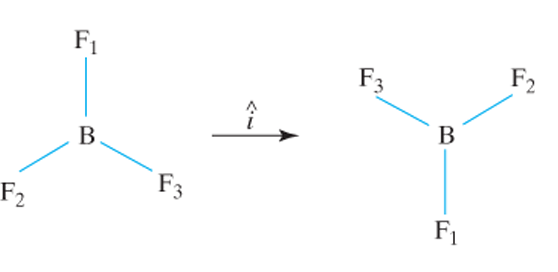
\includegraphics[width=0.5\textwidth]{Figures/12.3.png}\caption{\ce{BF_3}的对称中心反演过程。}
        \label{fig:12.3}
    \end{figure}
    \begin{figure}[htbp]
        \centering
        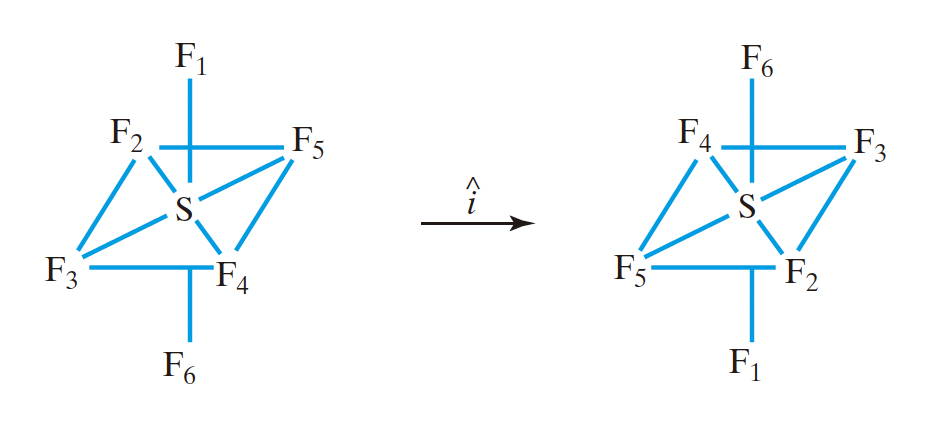
\includegraphics[width=0.5\textwidth]{Figures/12.4.png}\caption{\ce{SF_6}的对称中心反演过程。}
        \label{fig:12.4}
    \end{figure}

    第四和第五种对称元素为\textbf{$n$重旋转-反映对称轴}（$n$-fold rotation-reflection axis）（也称为\textit{反常轴}或\textit{象转轴}），记为$S_n$。若对具有$S_n$轴的物体进行$\left(360/n\right)$度的旋转，再通过该轴的垂直平面进行反射，则得到的构型与原始构型在物理上无法区分。显然，若某物体有$C_n$轴，也有与该轴垂直的反映面，那么该$C_n$轴也是一根$S_n$轴。因此，\ce{BF_3}中的$C_3$轴也是一根$S_3$轴。但$S_n$轴不一定是$C_n$轴。例如分子\ce{CH_4}。在图\ref{fig:12.5}中，我们首先进行了一次$90°$的正确旋转$\left(\hat{C}_4\right)$，围绕我们所认为的$S_4$轴。如图所示，得到的构型与原构型并不等价。当我们按照$\hat{C}_4$操作，在垂直于轴且通过碳原子的平面上进行反演时，我们确实得到了与旋转和反射之前存在的构型无法区分的构型。因此，\ce{CH_4}有一根$S_4$轴。$S_4$轴不是$C_4$轴，虽然它是一根$C_2$轴。甲烷分子中还有两个$S_4$轴，每条轴都垂直于四面体分子所内切的立方体的两条对边。
    \begin{figure}[htbp]
        \centering
        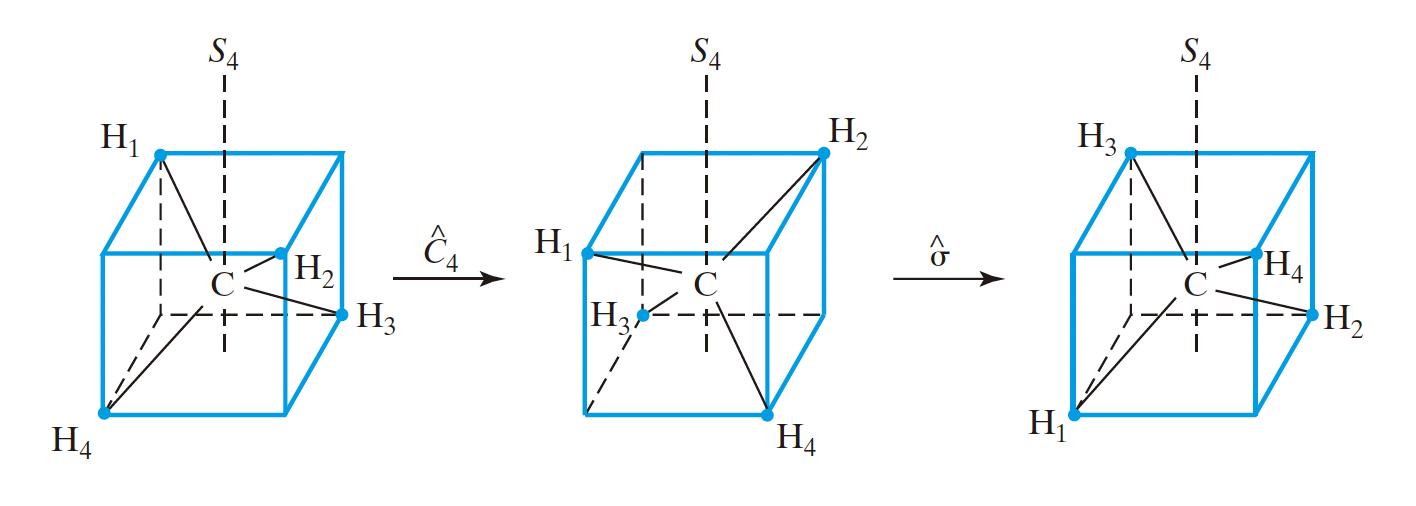
\includegraphics[width=0.55\textwidth]{Figures/12.5.png}\caption{\ce{CH_4}中的$S_4$轴。}
        \label{fig:12.5}
    \end{figure}
    \begin{figure}[htbp]
        \centering
        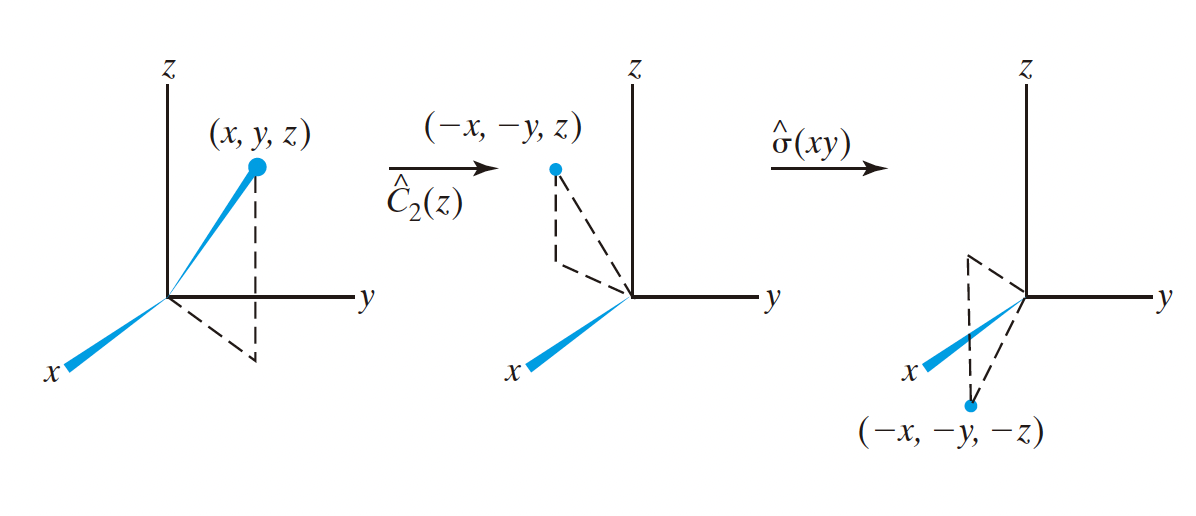
\includegraphics[width=0.55\textwidth]{Figures/12.6.png}\caption{$\hat{S}_n$操作。}
        \label{fig:12.6}
    \end{figure}

    绕轴逆时针旋转$\left(360/n\right)°$，再对垂直于此旋转轴的平面反映的操作记为$\hat{S}_n$。$\hat{S}_1$操作为绕该轴旋转$360°$后对垂直于该轴的平面进行反映。由于旋转$360°$回到了原来的位置，所以$\hat{S}_1$操作等价于对平面反映：$\hat{S}_1 = \hat{\sigma}$。一个反映面有一根与其垂直的$S_1$轴。

    现在来考虑$\hat{S}_2$操作。令$S_2$轴为$z$轴（图\ref{fig:12.6}）。绕$S_2$轴旋转$180°$使某点坐标$x$和$y$分别变为$-x$和$-y$，但$z$坐标保持不变。再以$xOy$平面作反映，将坐标$z$变为$-z$。$\hat{S}_2$操作的净结果为将坐标为$\left(x,y,z\right)$的点变为$\left(-x,-y,-z\right)$，相当于以原点为中心进行反演：$\hat{S}_2 = \hat{i}$。任何通过对称中心的轴都是一根$S_2$轴。平面反映和反演是$\hat{S}_n$操作的特例。

    $\hat{S}$操作似乎是一种任意的操作，但必须将其作为对称操作的一种类型包括在内。例如，图 \ref{fig:12.5} 中\ce{CH_4}从第一构型到第三构型的转换显然符合对称操作的定义，但它既不是正确的旋转，也不是反映或反演。

    对分子进行对称操作后，其核构型在物理上与原始构型无法区分。因此，对称操作前后，质心在空间中的位置必须相同。对于操作$\hat{C}_n$，唯一不动的点是位于$C$轴上的点。因此，$C_n$对称轴必须通过分子的质心。同样，对称中心必须与质心重合；对称平面和$S_n$对称轴必须通过质心。质心是所有分子对称元素的共同交点。

    在讨论分子的对称性时，我们通常将其置于笛卡尔坐标系中，并将分子的质心置于原点。最高阶的旋转轴被设定为$z$轴。包含该轴的对称平面被标记为$\sigma_v$（表示\textit{垂直，vertical}）；与该轴垂直的对称平面被标记为$\sigma_h$（表示\textit{水平，horizontal}）。

\subsection*{对称操作的乘积}

    对称操作是转换三维空间的算符，与任何算符一样，我们将两个此类算符的\textbf{乘积}（product）定义为连续应用这些算符，乘积右侧的算符先应用。显然，分子中任何两个对称操作的乘积必须是对称操作。

    例如，考虑分子\ce{BF_3}。$\hat{C}_3$操作与其自身的乘积$\hat{C}_3\hat{C}_3 = \hat{C}_3^2$将分子逆时针旋转$240°$。若我们取$\hat{C}_3\hat{C}_3\hat{C}_3 = \hat{C}_3^3$，则分子将逆时针旋转$360°$，回到原始位置。我们定义\textbf{恒等操作}（identity operation）为不对物体作任何变换的操作，记为$\hat{E}$。（该符号来自德语词\textit{Einheit}，意为单位。）

    现在再来考虑一个具有六重对称轴的分子，例如\ce{C_6H_6}。$\hat{C}_6$操作将分子逆时针旋转$60°$。$\hat{C}_6^2$将分子逆时针旋转$120°$，；因此$\hat{C}_6^2 = \hat{C}_3$。同样地，$\hat{C}_6^3 = \hat{C}_2$。因此，一根$C_6$对称轴也同时是一根$C_3$和$C_2$对称轴。

    对称算符总是可对易的吗？考虑\ce{SF_6}。我们检查绕$z$轴旋转的$\hat{C}_4$操作和绕$x$轴旋转$\hat{C}_2$操作的乘积。图\ref{fig:12.7}表明$\hat{C}_4\left(z\right)\hat{C}_2\left(x\right) \neq \hat{C}_2\left(x\right)\hat{C}_4\left(z\right)$。对称操作并不总是可对易的。请注意，我们描述的是相对于固定坐标系的对称操作，该坐标系在执行对称操作时不会随分子一起移动。因此，当我们进行$\hat{C}_4\left(z\right)$操作时，$\hat{C}_2\left(x\right)$操作的轴并未随分子一起旋转。
    \begin{figure}[htbp]
        \centering
        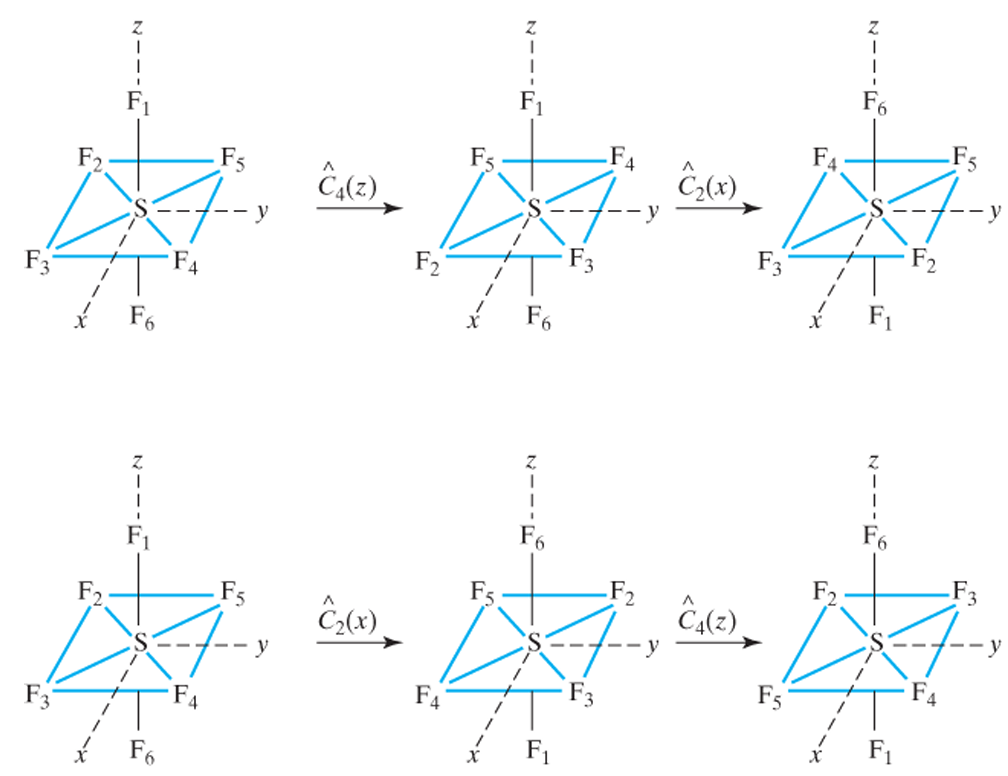
\includegraphics[width=0.65\textwidth]{Figures/12.7.png}\caption{
            \centering
            \parbox{0.5\textwidth}{
                \noindent
                \ce{SF_6}中两个对称操作的乘积。前三步：$\hat{C}_2\left(x\right)\hat{C}_4\left(z\right)$；后三步：$\hat{C}_4\left(z\right)\hat{C}_2\left(x\right)$。
            }
        }
        \label{fig:12.7}
    \end{figure}

\subsection*{对称性与偶极矩}

    作为对称性的应用，我们考虑分子偶极矩。由于对称操作会产生与原始构型在物理上无法区分的构型，因此对称操作后偶极矩矢量的方向必须保持不变。（这是一个不严谨、不复杂的论点。）因此，若我们有一根$C_n$对称轴，则偶极矩矢量必须与该轴重合。如果分子具有两根或更多不重合的对称轴，则该分子不能具有偶极矩，因为偶极矩不能位于两根不同的轴上。具有四根非重合对称轴的\ce{CH_4}分子就没有偶极矩。若存在反映面，则偶极矩矢量必须位于该反映面上。若有多个反映面，则偶极矩必须位于所有反映面的交线上。在分子\ce{H_2O}中，偶极矩矢量位于$C_2$轴上，该轴也是两个反映面的交线（图\ref{fig:12.8}）。具有对称中心的分子不能有偶极矩，因为反演操作反转了偶极矩的方向。（该表述有一种例外，见问题14.4。）因此，我们可以使用对称性来判断某分子是否具有偶极矩。在许多情况下，对称性还告诉我们偶极矩沿着哪条直线分布。
    \begin{figure}[htbp]
        \centering
        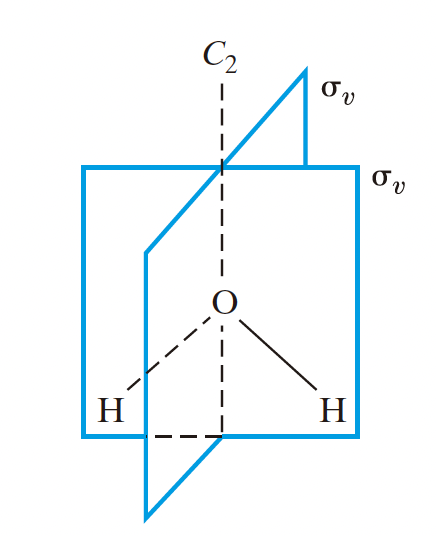
\includegraphics[width=0.25\textwidth]{Figures/12.8.png}
        \caption{\ce{H_2O}中的对称元素。}
        \label{fig:12.8}
    \end{figure}

\subsection*{对称性与旋光性}

    某些分子会使通过它们的平面偏振光的偏振平面发生旋转。实验证据和量子力学处理（\textit{Kauzmann}，pp. 703-713）表明，两个互为镜像的分子的旋光能力大小相等，符号相反。因此，如果一个分子是其自身的镜像，则它没有旋光性：$\alpha = -\alpha,\:2\alpha = 0,\: \alpha = 0$，其中$\alpha$为旋光率。如果一个分子不能与它的镜像重合，它可能具有旋光性。如果镜像分子的构象与原分子可以仅通过围绕一根旋转能垒较低的键进行旋转互换，那么该分子将不具有旋光性。

    对称性与旋光性之间的关系是什么呢？考虑$\hat{S}_n$操作。它包含了旋转$\left(\hat{C}_n\right)$和反映$\left(\hat{\sigma}\right)$操作。$\hat{S}_n$操作中的反映部分将分子转换为其镜像，若$\hat{S}_n$是该分子的对称操作，则$\hat{C}_n$操作将使分子与其镜像相重合：
    \begin{equation*}
        \text { 分子 } \stackrel{\hat{C}_{n}}{\rightarrow} \text { 镜像分子 } \stackrel{\hat{\sigma}}{\rightarrow} \text { 旋转镜像分子 }
    \end{equation*}
    因此，具有$S_n$对称轴的分子不能具有旋光性。若分子没有$S_n$对称轴，则它可能具有旋光性。

    因为$\hat{S}_1 = \hat{\sigma}$以及$\hat{S}_2 = \hat{i}$，所以具有对称中心或反映面的分子不能具有旋光性。然而，具有任意阶的$S_n$轴的分子都不会有旋光性。

    一个分子可以具有对称元素，同时仍具有旋光性。如果存在$C_n$轴而没有$S_n$轴，该分子可以具有旋光性。

\subsection*{对称操作与量子力学}

    分子的对称操作与量子力学之间有什么关系？为了对量子力学系统的状态进行分类，我们考虑与哈密顿算符以及彼此可对易的算符。例如，我们使用与算符$\hat{L}^2$、$\hat{S}^2$、$\hat{J}^2$、$\hat{M}_J$相对应的量子数 $L$、$S$、$J$ 和 $M_J$ 对多电子原子的状态进行了分类，所有这些算符都互相可对易，也可与哈密顿算符对易（忽略自旋-轨道耦合）。本章讨论的对称操作作用于三维空间中的\textit{点}，将每个点转换为相应的点。我们讨论过的所有量子力学算符都作用于\textit{函数}，将每个函数转换为相应的函数。与对称操作$\hat{R}$相对应，我们定义一个算符$\hat{O}_R$以如下方式作用于函数。令$\hat{R}$将某点从原来的位置$\left(x,y,z\right)$变换到$\left(x',y',z'\right)$：
    \begin{equation}
        \hat{R}\left(x,y,z\right) \to \left(x',y',z'\right)
        \label{eq:12.1}
    \end{equation}
    算符$\hat{O}_R$定义为函数$\hat{O}_Rf$在点$\left(x',y',z'\right)$的值与函数$f$在点$\left(x,y,z\right)$的值相等：
    \begin{equation}
        \hat{O}_Rf\left(x',y',z'\right) = f\left(x,y,z\right)
        \label{eq:12.2}
    \end{equation}

    例如，设$\hat{R}$为绕$z$轴旋转$90°$：$\hat{R} = \hat{C}_4\left(z\right)$；设$f$为氢$2p_x$轨道：$f = 2p_x = Nx\mathrm{e}^{-k\left(x^2+y^2+z^2\right)^{1/2}}$。$2p_x$轨道形状由绕$x$轴旋转的两个扭曲的椭球体组成（第\ref{sec:6.7 Hydrogenlike orbitals}节）。令这些椭球体的以点$\left(a,0,0\right)$和$\left(-a,0,0\right)$为“中心”，其中在右椭球中有$a>0$和$2p_x>0$。算符$\hat{C}_4\left(z\right)$具有如下效果（图\ref{fig:12.9}）：
    \begin{equation}
        \hat{C}_4\left(z\right)\left(x,y,z\right) \to \left(-y,x,z\right)
        \label{eq:12.3}
    \end{equation}
    例如，原本位于$\left(a,0,0\right)$的点在$\hat{C}_4\left(z\right)$操作后变为$\left(0,a,0\right)$，而$\left(-a,0,0\right)$变为$\left(0,-a,0\right)$。根据(\ref{eq:12.2})，函数$\hat{O}_{C_4\left(z\right)}2p_x$的轮廓必须分别以$\left(0, a, 0\right)$和$\left(0,-a,0\right)$为中心。因此，有（图\ref{fig:12.10}）：
    \begin{equation}
        \hat{O}_{C_4\left(z\right)}2p_x = 2p_y
        \label{eq:12.4}
    \end{equation}
    \begin{figure}[htbp]
        \centering
        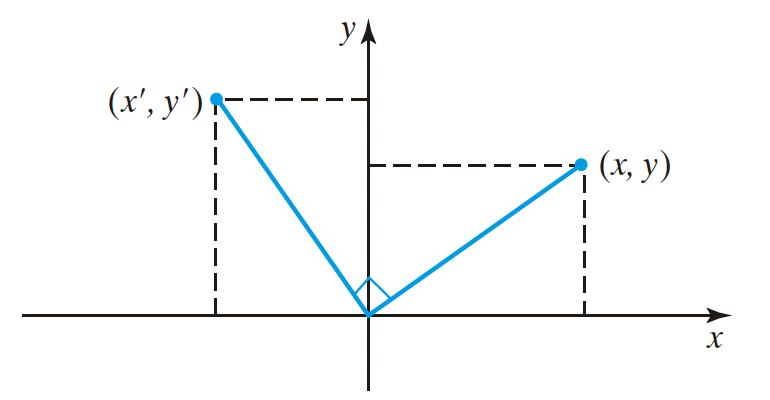
\includegraphics[width=0.45\textwidth]{Figures/12.9.png}
        \caption{
            \centering
            \parbox{0.4\textwidth}{
                \noindent
                $\hat{C}_4\left(z\right)$旋转的作用是将点$\left(x,y,z\right)$变为$\left(-y,x,z\right)$。使用三角函数可以看出$x'=-y$，$y'=-x$。
            }
        }
        \label{fig:12.9}
    \end{figure}
    \begin{figure}[htbp]
        \centering
        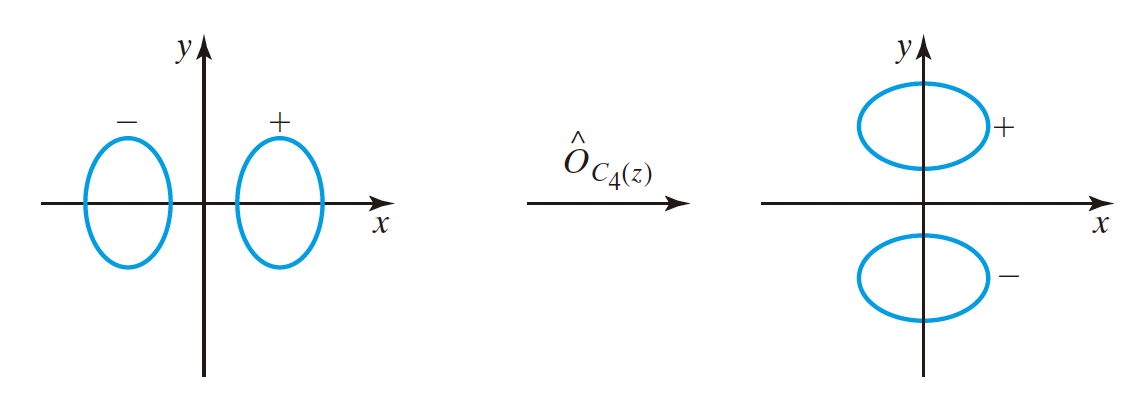
\includegraphics[width=0.7\textwidth]{Figures/12.10.png}
        \caption{$\hat{C}_4\left(z\right)$作用于$p_x$轨道的效果。}
        \label{fig:12.10}
    \end{figure}

    对于反演操作，我们有
    \begin{equation}
        \hat{i}\left(x,y,z\right) \to \left(-x,-y,-z\right)
        \label{eq:12.5}
    \end{equation}
    根据(\ref{eq:12.2})，有
    \begin{equation*}
        \hat{O}_i f\left(-x,-y,-z\right) = f\left(x,y,z\right)
    \end{equation*}
    我们现在重新命名变量：$\bar{x} = -x$，$\bar{y} = -y$，$\bar{z} = -z$。因此，
    \begin{equation*}
        \hat{O}_i f\left(\bar{x},\bar{y},\bar{z}\right) = f\left(-\bar{x},-\bar{y},-\bar{z}\right)
    \end{equation*}
    点$\left(\bar{x}, \bar{y}, \bar{z}\right)$是空间中的任意一点，因此我们可以去掉字母上的横杆，得到
    \begin{equation*}
        \hat{O}_i f\left(x,y,z\right) = f\left(-x,-y,-z\right)
    \end{equation*}
    因此，$\hat{O}_i$为宇称算符（第\ref{sec:7.5 Parity}节）：$\hat{O}_i = \hat{\Pi}$。

    $n$粒子系统的波函数是$4n$个变量的函数，我们展开$\hat{O}_R$的定义(\ref{eq:12.2})，得到
    \begin{equation*}
        \hat{O}_Rf\left(x_1',\:y_1',\:z_1',\:m_{s1},\:\ldots,\:x_n',\:y_n',\:z_n',\:m_{sn}\right) = f\left(x_1,\:y_1,\:z_1,\:m_{s1},\:\ldots,\:x_n,\:y_n,\:z_n,\:m_{sn}\right)
    \end{equation*}
    注意$\hat{O}_R$并不影响自旋坐标。因此，在第\ref{sec:11.5 Angular momentum in Many-Electron Atoms}节中讨论原子态的宇称时，我们考察了斯莱特行列式展开式中各项的空间因子，而未考虑自旋因子，因为这些因子不受$\hat{\Pi}$的影响。

    若某系统由对称操作$\hat{R}_1,\:\hat{R}_2,\:\ldots$指定，则相对应的算符$\hat{O}_{R_1},\:\hat{O}_{R_2},\:\ldots$都与哈密顿算符可对易。（证明见\textit{Schonland}, Section 7.1-7.3.）例如，如果分子的核框架具有对称中心，则宇称算符 $\hat{\Pi}$ 与电子运动的哈密顿算符可对易。根据$\hat{\Pi}$的本征值，我们可以选择电子态（波函数）为奇函数或偶函数。当然，并非所有的对称操作都能对易（图\ref{fig:12.7}）。因此，波函数通常不能被选作所有对称算符 $\hat{O}_R$ 的本征函数。（对称算符和分子波函数之间关系的进一步讨论见第\ref{sec:15.2 Electronic Terms of Polyatomic Molecules}节。）

    对称性与\textit{运动常数}之间有着密切的联系（这些常数是与哈密顿算符 $\hat{H}$ 可对易的属性）。对于哈密顿算符在任何空间坐标平移下都恒定（即不变）的系统，线动量算符 $\hat{p}$ 将与 $\hat{H}$ 可对易，并且 $p$ 在定态下可以被赋予一个确定的值。自由粒子就是一个例子。对于在任何坐标旋转下 $\hat{H}$ 不变的系统，角动量分量的算符与 $\hat{H}$ 可对易，总角动量及其一个分量可以指定。一个例子是原子。线性分子具有轴对称性，而不是原子的球对称性；在这里，只能指定角动量的轴向分量（第 \ref{chap:13} 章）。

\subsection*{矩阵与对称操作}

    对称操作$\hat{R}$将原来处于$x,y,z$的点移动到新的位置$x',y',z'$，其中每个$x',y',z'$都是$x,y,z$的线性组合（证明见\textit{Schonland}, pp. 52-53.）：
    \begin{equation*}
        \begin{aligned}
            x' &= r_{11}x + r_{12}y + r_{13}z \\
            y' &= r_{21}x + r_{22}y + r_{23}z \\
            z' &= r_{31}x + r_{32}y + r_{33}z
        \end{aligned} \quad \text{或} \quad
        \begin{pmatrix}
            x' \\
            y' \\
            z'
        \end{pmatrix}
        =\begin{pmatrix}
            r_{11} & r_{12} & r_{13} \\
            r_{21} & r_{22} & r_{23} \\
            r_{31} & r_{32} & r_{33}
        \end{pmatrix}\begin{pmatrix}
            x \\
            y \\
            z
        \end{pmatrix}
    \end{equation*}
    其中$r_{11},\:r_{12},\:\ldots,\:r_{33}$是常数，其值取决于$\hat{R}$的性质。我们说对称操作$\hat{R}$可以\textbf{表示}（represented）成元素为$r_{11},\:r_{12},\:\ldots,\:r_{33}$的矩阵$\mathbf{R}$。由矩阵$\mathbf{R}$描述变换的函数组$x,\:y,\:z$称为该表示的\textbf{基}（basis）。

    例如，由(\ref{eq:12.3})和(\ref{eq:12.5})，对于操作$\hat{C}_4\left(z\right)$，我们有$x' = -y,\: y' = x,\: z' = z$。以$x,\:y,\:z$为基，$\hat{C}_4\left(z\right)$和$\hat{i}$的矩阵表示为
    \begin{equation*}
        \mathbf{C}_4\left(z\right) = \begin{pmatrix}
            0 & -1 & 0 \\
            1 & 0 & 0 \\
            0 & 0 & 1
        \end{pmatrix}, \quad \mathbf{i} = \begin{pmatrix}
            -1 & 0 & 0 \\
            0 & -1 & 0 \\
            0 & 0 & -1
        \end{pmatrix}
    \end{equation*}
    若两个对称操作$\hat{R}\hat{S}$的乘积为$\hat{T}$，则它们以$x,\:y,\:z$为基的矩阵以相同的方式相乘；即：若$\hat{R}\hat{S} = \hat{T}$，则$\mathbf{R}\mathbf{S} = \mathbf{T}$。（证明见\textit{Schonland}, pp. 56-57.）。

\section{对称点群}
\label{sec:12.2 Symmetry Point Groups}

    现在，我们来考虑对称元素可能的组合。分子中不能出现对称元素的任意组合。例如，假设某分子有且仅有一根$C_3$轴。任何对称操作都必须使该轴保持不变。因此，该分子不能有与$C_3$轴呈任意角度的反映面，任何反映面必须包含该轴或与该轴垂直。（\ce{BF_3}中有三个$\sigma_v$面和一个$\sigma_h$面。）某对称轴与$C_3$轴不重合的唯一可能是与$C_3$轴垂直的$C_2$轴。对应的$\hat{C}_2$操作使$C_3$轴保持不变。因为$\hat{C}_3$和$\hat{C}_3^2$是对称操作，若有一根垂直于$C_3$轴的$C_2$轴，则必须同时有六根$C_2$轴（与\ce{BF_3}中的情况相同）。

    分子中所有的对称操作构成一个数学意义上的群。\textbf{群}（group）是一个由实体【称为群的\textbf{元素}（elements）或\textbf{成员}（members）】组成的集合，以及一条将群中的任意两个元素结合以形成这些元素的积的规则，使得某些要求得到满足。令$A,\:B,\:C,\:D,\:\ldots$（假设互不相等）为某群的元素，令$B \ast C$为$B$与$C$的积。乘积$B \ast C$不一定与$C \ast B$相等。群的元素必须满足以下要求：(1)任意两个元素的乘积（包括某元素与其自身）都必须是该群的元素之一【\textbf{封闭性}（closure）】；(2)群中必须存在\textbf{恒等元素}（identity element），使得对群中的每个元素$K$都有$K \ast I = K$和$I \ast K = K$；(3)群中每个元素$K$必须有一个\textbf{逆元素}（inverse element）$K^{-1}$，使得$K \ast K^{-1} = I$和$K^{-1} \ast K = I$，其中$I$为恒等元素；(4)群的乘积满足\textbf{结合律}（associative），即对任意群都有$\left(B \ast D\right) \ast G = B \ast \left(D \ast G\right)$。

    群中元素的个数称为群的\textbf{阶}（order）。若对群中任意两个元素都有$B \ast C = C \ast B$，则称该群为\textbf{交换群或阿贝尔群}（commutative or Abelian group）。

    群的一个例子是所有整数（正数、负数和零）的集合，其运算规则为普通的加法。因为两个整数的和仍是整数，所以封闭性成立。其恒等元素是$0$。整数$n$的逆元素为$-n$。以及加法满足结合律。该群是一个无穷阶阿贝尔群。

    在$\hat{R}$和$\hat{S}$的组合为连续应用$\hat{R}$和$\hat{S}$的规则下，三维物体的所有对称操作集合构成一个群。因为两个对称操作的乘积一定是对称操作，则封闭性成立。该群的恒等元素为恒等操作$\hat{E}$，即不作任何操作。结合律也满足【式(\ref{eq:3.6 law of multiplication for operators})】。对称操作$\hat{R}$的逆元素为撤销$\hat{R}$的操作，例如，因为$\hat{i}\hat{i} = \hat{E}$，则反演操作$\hat{i}$的逆元素就是它本身。逆时针旋转$120°$操作$\hat{C}_3$的逆元素是顺时针旋转$120°$操作，等价于逆时针旋转$240°$，则$\hat{C}_3^{-1} = \hat{C}_3^2$以及$\hat{C}_3\hat{C}_3^2 = \hat{E}$。\textit{请注意，该群的成员（元素）是分子的对称操作（而不是对称元素）。}我们在第\ref{sec:15.2 Electronic Terms of Polyatomic Molecules}节中将使用一些群论知识，但群论的完整发展及其应用在此省略（参见\textit{Cotton}或\textit{Schonland}）。

    对分子所作的任何对称操作，质心点都保持不变。因此，孤立分子的对称群被称为\textbf{点群}（point group）。对于无限大的晶体，我们可以进行对称操作（例如平移），但这些操作不会使任何点保持不变，从而产生\textit{空间群}（space group）。本书省略了对空间群的讨论。

    每个分子都属于我们现在列出的对称点群之一。为了方便起见，点群已被分为四个类别。花体字母表示点群。

    \begin{center}
        I. \textit{不具有$C_n$轴的点群：$\mathscr{C}_1$、$\mathscr{C}_s$和$\mathscr{C}_i$。}
    \end{center}
    \begin{enumerate}
        \item $\mathscr{C}_1$：若某分子不具有任何对称元素，则它属于该点群。唯一的对称操作为$\hat{E}$（也是$\hat{C}_1$旋转操作）。分子\ce{CHFClBr}属于点群$\mathscr{C}_1$。
        \item $\mathscr{C}_s$：具有唯一对称元素为反映面的分子属于该点群。对称操作为$\hat{E}$和$\hat{\sigma}$。一个例子为\ce{HOCl}（图\ref{fig:12.11}）。
        \item $\mathscr{C}_i$：具有唯一对称元素为对称中心的分子属于该点群。对称操作为$\hat{E}$和$\hat{i}$。
    \end{enumerate}
    \begin{figure}[ht]
        \centering
        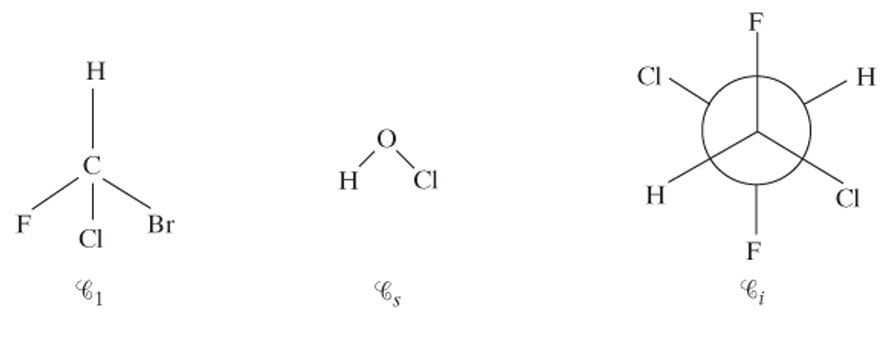
\includegraphics[width=0.65\textwidth]{Figures/12.11.png}
        \caption{不具有$C_n$轴的分子。}
        \label{fig:12.11}
    \end{figure}
    \begin{figure}[ht]
        \centering
        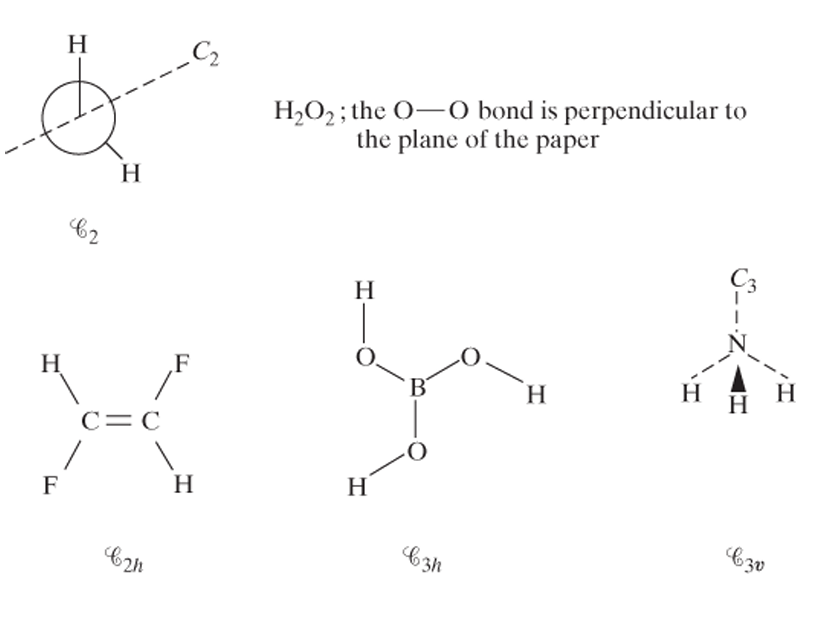
\includegraphics[width=0.6\textwidth]{Figures/12.12.png}
        \caption{只有一根$C_n$轴的分子。}
        \label{fig:12.12}
    \end{figure}

    \begin{center}
        II. \textit{只有一根$C_n$轴的点群：$\mathscr{C}_n$、$\mathscr{C}_{nh}$和$\mathscr{C}_{nv}$和$\mathscr{S}_{2n}$。}
    \end{center}
    \begin{enumerate}
        \item $\mathscr{C}_n, \: n = 2,\:3,\:4,\:\ldots$：只具有一根$C_n$旋转轴的分子属于该点群。对称操作为$\hat{C}_n,\: \hat{C}_n^2,\:\ldots,\:\hat{C}_n^{n-1},\:\hat{E}$。属于$\mathscr{C}_2$点群的分子如图\ref{fig:12.12}所示。
        \item $\mathscr{C}_{nh}, \: n = 2,\:3,\:4,\:\ldots$：若我们添加一个垂直于$C_n$轴的反映面，则得到了属于该点群的分子。因为$\hat{\sigma}_h\hat{C}_n = \hat{S}_n$，所欲对称轴$C_n$也是$S_n$轴。若$n$为偶数，则$C_n$轴也是$C_2$轴，分子具有对称操作$\hat{\sigma}_h\hat{C}_2 = \hat{S}_2 = \hat{i}$。因此，若$n$为偶数，则属于$\mathscr{C}_{nh}$点群的分子具有对称中心。（群$\mathscr{C}_{1h}$即之前讨论过的群$\mathscr{C}_s$。）属于点群$\mathscr{C}_{2h}$和$\mathscr{C}_{3h}$的分子如图\ref{fig:12.12}所示。
        \item $\mathscr{C}_{nv}, \: n = 2,\:3,\:4,\:\ldots$：属于该点群的分子有一根$C_n$轴，以及$n$个通过$C_n$轴的垂直反映面。（群$\mathscr{C}_{1v}$为群$\mathscr{C}_s$。）\ce{H_2O}具有一根$C_2$轴和两个通过该轴的反映面，属于$\mathscr{C}_{2v}$点群。\ce{NH_3}分子属于$\mathscr{C}_{3v}$点群。（见图\ref{fig:12.12}。）
        \item $\mathscr{S}_n, \: n = 4,\:6,\:8,\:\ldots$：$\mathscr{S}_n$点群是与$S_n$轴有关的点群。首先考虑$n$为级数的情况。我们有$\hat{S}_n = \hat{\sigma}_h\hat{C}_n$。操作$\hat{C}_n$只影响$x$和$y$坐标，而$\hat{\sigma}_h$操作只影响$z$坐标。因此，这些操作可以对易，我们有
        \begin{equation*}
            \hat{S}_{n}^{n} = (\hat{\sigma}_{h} \hat{C}_{n})^{n} = \hat{\sigma}_{h} \hat{C}_{n} \hat{\sigma}_{h} \hat{C}_{n} g \hat{\sigma}_{h} \hat{C}_{n} = \hat{\sigma}_{h}^{n} \hat{C}_{n}^{n}
        \end{equation*}
        现在$\hat{C}_{n}^{n} = \hat{E}$，以及对奇数$n$，有$\hat{\sigma}_{h}^{n} = \hat{\sigma}_{h}$。因此对于奇数$n$，对称操作$\hat{S}_n^n$等价于$\hat{\sigma}_h$，以及点群$\mathscr{S}_n$具有水平反映面。同样地，
        \begin{equation*}
            \hat{S}_{n+1} = \hat{S}_{n}\hat{S}_{n} = \hat{\sigma}_{h} \hat{S}_{n} = \hat{\sigma}_{h} \hat{\sigma}_{h} \hat{C}_{n} = \hat{C}_{n}, \quad n \text{ odd}
        \end{equation*}
        所以若$n$为奇数，则分子具有一根$C_2$轴。因此，若$n$为奇数，$\mathscr{S}_n$群等价于$\mathscr{C}_{nh}$群。再考虑$n$为偶数的情况。因为$\hat{S}_2=\hat{i}$，则群$\mathscr{S}_2$等价于$\mathscr{C}_i$。因此只有当$n = 4,\:6,\:8,\:\ldots$时，$\mathscr{S}_n$群才是一个新的点群。$S_{2n}$轴也是$C_n$轴：$\hat{S}_{2n}^2 = \hat{\sigma}_h^2 \hat{C}_{2n}^2 = \hat{E}\hat{C}_n = \hat{C}_n$。
    \end{enumerate}

    \begin{center}
        III. \textit{具有一根$C_n$轴和$n$个$C_2$轴的点群：$\mathscr{D}_n$、$\mathscr{D}_{nh}$和$\mathscr{D}_{nd}$。}
    \end{center}
    \begin{figure}[ht]
        \centering
        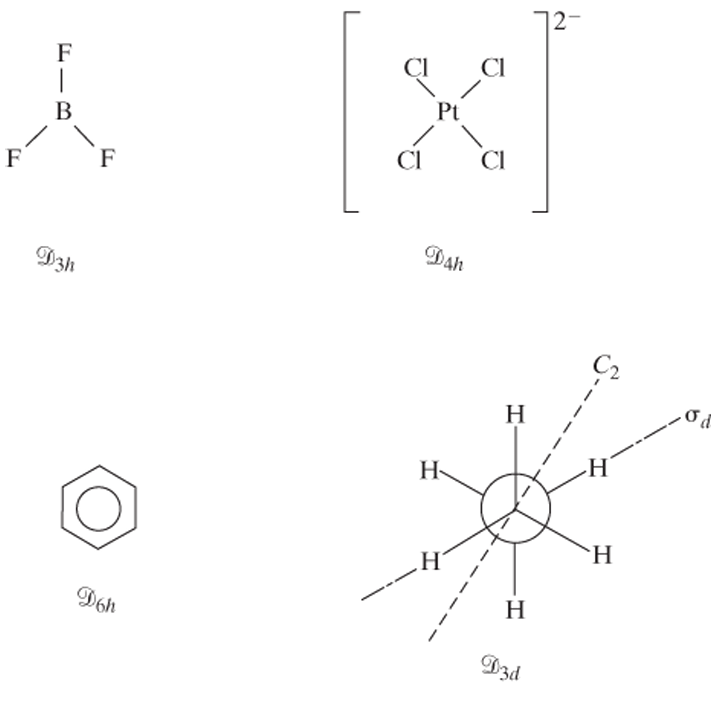
\includegraphics[width=0.5\textwidth]{Figures/12.13.png}
        \caption{具有一根$C_n$轴和$n$个$C_2$轴的分子。}
        \label{fig:12.13}
    \end{figure}
    \begin{enumerate}
        \item $\mathscr{D}_n, \: n = 2,\:3,\:4,\:\ldots$：具有一根$C_n$轴和$n$根与$C_n$轴垂直的$C_2$轴（不存在反映面）的分子属于该点群。相邻$C_2$轴之间的夹角为$\pi/n$弧度。$\mathscr{D}_2$点群有三根互相垂直的$C_2$轴，对称操作为$\hat{E}, \:\hat{C}_2(x), \:\hat{C}_2(y), \:\hat{C}_2(z)$。
        \item $\mathscr{D}_{nh}, \: n = 2,\:3,\:4,\:\ldots$：具有一根$C_n$轴、$n$根$C_2$轴和一个垂直于$C_n$轴的反映面$\sigma_h$的分子属于该点群。与$\mathscr{C}_{nh}$一致，$C_n$轴也是$S_n$轴。若$n$为偶数，则$C_n$轴也是$C_2$轴和$S_2$轴，分子具有对称中心。$\mathscr{D}_{nh}$群中的分子也有$n$个反映面，每个都穿过$C_n$轴和其中一根$C_2$轴。（证明见问题12.29。）\ce{BF_3}分子属于$\mathscr{D}_{3h}$点群；\ce{PtCl_4^2-}属于$\mathscr{D}_{4h}$点群；苯属于$\mathscr{D}_{6h}$点群（图\ref{fig:12.13}）。
        \item $\mathscr{D}_{nd}, \: n = 2,\:3,\:4,\:\ldots$：具有一根$C_n$轴、$n$根$C_2$轴和$n$个通过$C_n$轴且平分相邻$C_2$轴夹角的反映面的分子属于该点群。$n$个垂直反映面称为\textbf{等分}（diagonal）平面，用$\sigma_d$表示。可以证明，$C_n$轴也是$S_{2n}$轴。乙烷交叉构象是$\mathscr{D}_{3d}$点群的典型例子（图\ref{fig:12.13}）。【具有内旋转的分子（例如乙烷）的对称性实际上需要特别考虑；见H. C. Longuet-Higgins, \textit{Mol. Phys.}, \textbf{6}, 445 (1963).】
    \end{enumerate}

    \begin{center}
        IV. \textit{具有多根$C_n$轴的点群，$n>2$：$\mathscr{T}_d,\: \mathscr{T},\: \mathscr{T}_h,\: \mathscr{O}_h,\: \mathscr{O},\: \mathscr{I}_h,\: \mathscr{I},\: \mathscr{K}_h$。}
    \end{center}
    \begin{figure}[ht]
        \centering
        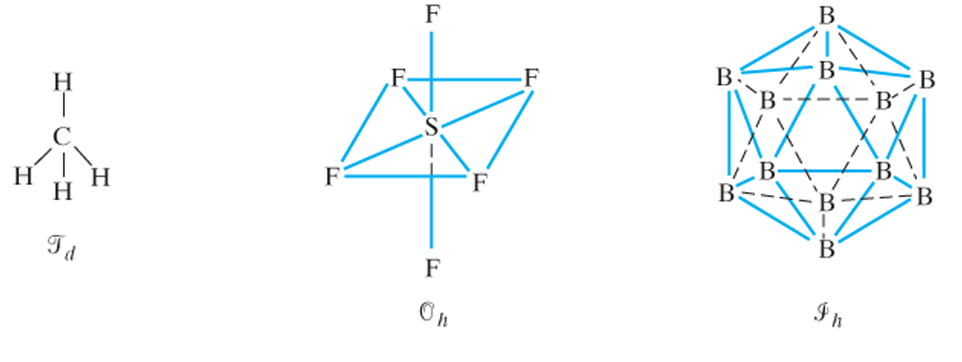
\includegraphics[width=0.7\textwidth]{Figures/12.14.png}
        \caption{
            \centering
            \parbox{0.5\textwidth}{
                \noindent
                具有多根$C_n$轴的点群，$n>2$。（对于\ce{B_12H_12^2-}，为了清晰起见，氢原子省略了。）
            }
        }
        \label{fig:12.14}
    \end{figure}
    这些立体与柏拉图立体的对称性有关，即由全等正多边形围成的立体，且具有全等的多面体角。共有五种这样的立体：四面体有四个三角形面，立方体有六个正方形面，八面体有八个三角形面，五角十二面体有十二个五边形面，二十面体有二十个三角形面。
    \begin{enumerate}
        \item $\mathscr{T}_d$：正四面体的对称操作构成了这个群。最典型的例子是\ce{CH_4}。甲烷的对称元素为四根$C_3$轴（每根\ce{C-H}键）、三根同时是$C_2$轴的$S_4$轴（图\ref{fig:12.5}）以及六个反映面，每个包含两根\ce{C-H}键。（从4个事物中每次取2个的组合数为$4!/2!\:2! = 6$。）
        \item $\mathscr{O}_h$：立方体或正八面体的对称操作构成了这个群。立方体和八面体被称为彼此的\textit{对偶}（dual）体；如果我们将立方体相邻面的中点连接起来，就会得到一个八面体，反之亦然。因此，立方体和八面体具有相同的对称元素和操作。立方体有六个面、八个顶点和十二条边。它的对称元素如下：一个对称中心、三根穿过立方体相对两面中心点的$C_4$轴（同时也是$S_4$和$C_2$轴）、四根穿过立方体对角的$C_3$轴（同时也是$S_6$轴）、六根连接一对相对边中点的$C_2$轴，三个与一对相对面平行的反映面以及六个通过一对相对边中点的反映面。八面体分子例如\ce{SF_6}属于$\mathscr{O}_h$点群。
        \item $\mathscr{I}_h$：正五角十二面体或正二十面体（彼此对偶）的对称操作构成了这个群。离子\ce{B_12H_12^2-}属于点群$\mathscr{I}_h$。十二个硼原子位于正二十面体的顶点上（图\ref{fig:12.14}）。足球形状的分子\ce{C_60}（富勒烯）也属于该点群。其形状为截角二十面体，通过切除正二十面体（图\ref{fig:12.14}）的12个顶点而成，从而生成一个具有12个五边形面（每个原二十面体的顶点处有5个面相交）、20个六边形面（由原正二十面体的20个三角形面形成），以及$12\times5=60$个顶点（切除原正二十面体的一个顶点后会产生5个新顶点）的图形。
        \item $\mathscr{K}_h$：这是球体的对称操作群。（\textit{Kugel}在德语中“球体”的意思。）原子属于这个群。
    \end{enumerate}

    完整起见，我们提及了与柏拉图立体相关的其他群，这些群在化学上并不重要。群$\mathscr{T}$、$\mathscr{O}$和$\mathscr{I}$分别是四面体、立方体和二十面体的正旋转对称群。这些群没有这些立体的对称反射和非正常旋转，也没有立方体和二十面体的反演操作。群$\mathscr{T}_h$包含四面体的对称旋转、反演操作以及某些反射和非正常旋转。

    线性分子属于什么群呢？围绕线性分子的核间轴进行任意角度的旋转是一种对称操作。$n$正多边形具有一根$C_n$轴，取极限$n \to \infty$，我们就得到了圆，圆有一根$C_{\infty}$轴。因此，线性分子的核间轴为$C_{\infty}$轴。任何包含此轴的面都是反映面。若线性分子不具有对称中心（例如\ce{CO}，\ce{HCN}），它属于点群$C_{\infty v}$。若线性分子具有对称中心（例如\ce{H_2}，\ce{C_2H_2}），则它具有$\sigma_h$反映面，即无穷多根垂直于分子主轴的$C_2$轴，因此属于点群$D_{\infty h}$。

    我们如何寻找分子所属点群？一种方法是找出所有的对称元素，与上述列出的点群进行比较。另一种更系统的方法如图\ref{fig:12.15}所述。【J. B. Calvert, \textit{Am. J. Phys.}, \textbf{31}, 659 (1963)。】该方法基于点群的四个分类。
    \begin{figure}[ht]
        \centering
        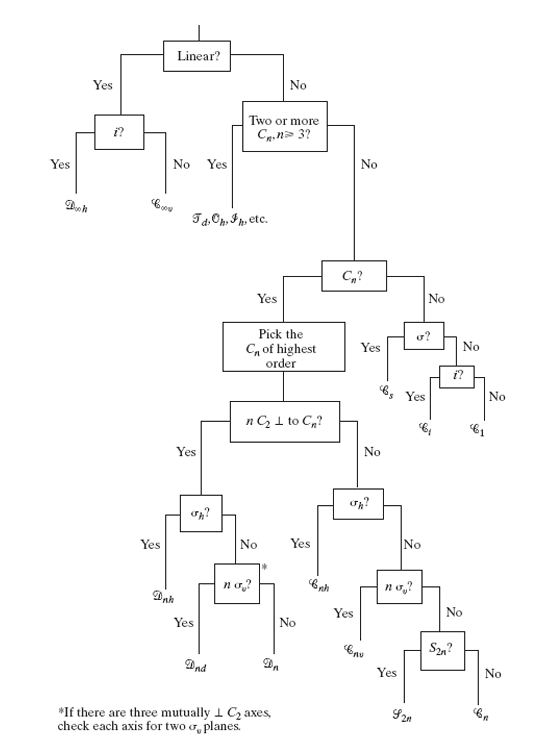
\includegraphics[width=0.7\textwidth]{Figures/12.15.png}
        \caption{确定分子所属点群步骤示意图。}
        \label{fig:12.15}
    \end{figure}

    首先，判断分子是否为线性分子。根据线性分子是否有对称中心，可以分为$\mathscr{D}_{\infty h}$和$\mathscr{C}_{\infty v}$两类。若分子不是线性分子，则寻找是否有大于等于两根的三重或更高阶对称轴。若存在，该分子被归类于与正多面体对称性相关的点群之一（第IV组）。若这些轴不存在，我们寻找任意一根$C_n$轴。若不存在任何$C_n$轴，则分子属于点群$\mathscr{C}_s$、$\mathscr{C}_i$和$\mathscr{C}_1$之一（第I组）。若至少存在一根$C_n$轴，在进行下一步之前，先选择最高阶的$C_n$轴为主对称轴。（如果有三根互相垂直的$C_2$轴，可以任取一根为主轴。）接下来，我们检查与主$C_n$轴垂直的$n$根$C_2$副轴。若它们存在，则分子属于点群组III；若不存在，则属于点群组II。如果我们找到了$n$根$C_2$轴，再寻找与主$C_n$轴垂直的反映面。若存在，则点群为$\mathscr{D}_{nh}$；若不存在，寻找包含主$C_n$轴的$n$个反映面（若分子有三根互相垂直的$C_2$轴，那么在寻找两个$\sigma_v$面时，我们必须将每根轴作为主轴进行测试；在点群$\mathscr{D}_{nh}$和$\mathscr{D}_{n}$中，这三根$C_2$轴是等价的，但在$\mathscr{D}_{nd}$中不是。）若我们找到了$n$个$\sigma_v$面，则点群为$\mathscr{D}_{nd}$；否则为$\mathscr{D}_n$。若分子不具有与$C_n$轴垂直的$n$根$C_2$副轴，通过首先寻找$\sigma_h$反映面，然后$n$个$\sigma_v$反映面，若它们都没有，那么最终检查$C_n$轴是否也为$S_{2n}$轴，我们将其分类到点群$\mathscr{C}_{nh}$、$\mathscr{C}_{nv}$、$\mathscr{S}_{2n}$或$\mathscr{C}_n$中。图\ref{fig:12.15}所示的步骤并不能确定所有对称元素。在对分子进行分类后，需确认所有必要的对称元素确实存在。尽管上述步骤看似复杂，但实际上非常简单且易于记忆。
    \begin{figure}[ht]
        \centering
        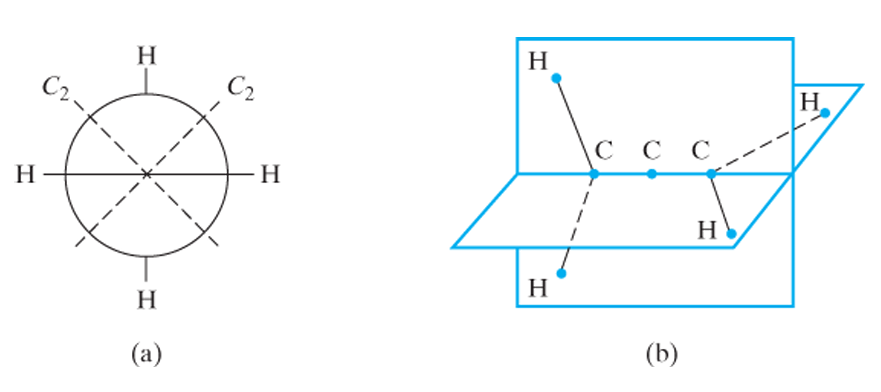
\includegraphics[width=0.6\textwidth]{Figures/12.16.png}
        \caption{联烯的两种视图。\ce{C=C=C}轴垂直于图(a)中纸张的平面。}
        \label{fig:12.16}
    \end{figure}

    学生在对分子进行归类时最常见的错误是忽略了属于$\mathscr{D}_{nd}$点群分子垂直于$C_n$主轴的$n$根$C_2$副轴。例如，我们很容易发现，联烯的\ce{C=C=C}轴是一根$C_2$轴，但另外两根$C_2$轴却很容易被忽视（图\ref{fig:12.16}）。具有两个相等且相互错开的半部分的分子通常属于$\mathscr{D}_{nd}$点群。例如，\ce{C_2H_2}分子具有两个$C_2$轴（图\ref{fig:12.16}）。模型可能对那些在可视化方面有困难的人有所帮助。

\section*{总结}

\section*{习题}